\documentclass[11pt]{article}
\usepackage[T1]{fontenc}
\usepackage[utf8]{inputenc}
\usepackage{multirow}
\usepackage{graphicx}
\graphicspath{ {img/} }
\usepackage[table,xcdraw]{xcolor}
\usepackage{listings}
\usepackage{hyperref}
\usepackage{pgfgantt}
\usepackage{vmargin}
\usepackage{wrapfig}
\usepackage{enumitem}
\usepackage{subfiles}
\usepackage{multirow}
\usepackage{float}
\usepackage{url}
\usepackage{makeidx}

\setlength\parindent{0pt}

\makeindex

\setpapersize{A4}
\setmargins{2.5cm}  % margen izquierdo
{1.5cm}             % margen superior
{16.5cm}            % anchura del texto
{23.42cm}           % altura del texto
{10pt}              % altura de los encabezados
{1cm}               % espacio entre el texto y los encabezados
{0pt}               % altura del pie de p�gina
{2cm}               % espaci\title{Determinitzaci� d'un aut�mat finit}


\definecolor{barblue}{RGB}{153,204,254}
\definecolor{groupblue}{RGB}{51,102,254}
\definecolor{linkred}{RGB}{165,0,33} 

\author{José Miguel Avellana López}
\date{25 de Marzo del 2021}

\def\contentsname{Index}
\begin{document}
	
	\setcounter{tocdepth}{4}
	\setcounter{secnumdepth}{4}
	
	\begin{titlepage}
		\begin{figure}[htb]
			\begin{center}
				
\includegraphics[width=7cm]{logoUDL.png}
				\vspace*{\stretch{1.0}}
				\\
				\medskip
				\begin{center}
					\noindent\rule{16.5cm}{0.4pt}
					\linebreak 
					\\
					\Huge\textbf {Sistema distribuido para la resolución de problemas SAT}
					\noindent\rule{16.5cm}{0.4pt}
					\hfill\\
					\Large\textbf\textit{Memoria}
					%\noindent\rule{16.5cm}{0.4pt}
					\\
					\bigskip
					\hfill\\
					\hfill\\
					\hfill\\
					\hfill\\
					\hfill\\
					\hfill\\
					\hfill\\
					\setlength{\parskip}{1em}
				\end{center}
				\vspace*{\stretch{2.0}}
			\end{center}
		\end{figure}
		\begin{flushright}
			Universitat de Lleida
			\\
			Escola Politécnica Superior
			\\
			Grau en Enginyeria Informática
			\\
			\medskip
			\hfill\\
			\normalsize\textbf{Autor:}
			\\
			\large\textit{Jose Miguel Avellana López}
			\\
			\normalsize\textbf{Codirector:}
			\\
			\large{Josep Luis Lérida Monsó}
			\\
			\normalsize\textbf{Codirector:}
			\\
			\large{Josep Argelich Romá}
		\end{flushright}
		\thispagestyle{empty} 
	\end{titlepage}
	\thispagestyle{empty}
	\newpage
		\renewcommand*\listfigurename{Index de figures}
		\thispagestyle{empty}
		\renewcommand*\listtablename{Index de taules}
		\thispagestyle{empty}
	\newpage
	
	\printindex

	\section{Introdución}
		\subsection{Contexto y motivación}
			En 1970, el matemático británico John Horton Conway diseño un automata celular al que llamo El Juego de la Vida.
			Un autómata celular es un modelo matemático y computacional para un sistema dinámico que evoluciona en pasos discretos.

			El juego de la vida viene a decir que, a partir de un conjunto de reglas simples, se pueden generar estructuras complejas.
			Un sistema compuesto de un conjunto de agentes ( o células), que ocupan un lugar en él, que poseen una serie de reglas 
			que definen como interaccionan con el resto de agentes.

			Y es que, en cierto modo, asi es como funciona la evolucion de un ecosistema de seres vivos, mejorando y optimizando sus procesos sin que exista
			una intención consciente de ello por parte de sus agentes.

			Bajo este mismo principio se puede entender la capacidad de los sistemas económicos basados en la competencia para mejorar sus procesos. 
			Cuando una empresa se dedica a investigar nuevas tecnologías para abaratar costes, no lo hace por el bien común, lo hace para vencer a sus rivales,
			pero, de manera inconsciente, sirve al bien común. Será el mercado el que dictará si esta nueva forma de realizar dicha tarea es más optima o no.

			Por lo tanto, es la competencia de ideas, de procesos y formas de actuación la que
			nos permite mejorar la forma en que vivimos.
			Teniendo en mente, por ejemplo, procesos industriales o logísticos, 
			si a alguien se le ocurre una forma más eficiente de hacer algo creará una empresa que realice esta labor en la manera que propone, 
			si realmente es mejor que el método tradicional, 
			terminará abarcando un cada vez mayor porcentaje de su mercado e imponiendose al método anterior. 

			Pero esta es una forma muy lenta de evolucionar debido a que el tiempo para observar resultados es el de un escenario real.
			Sin embargo, podemos observar nuevas propuestas de actuación en entornos simulados, en mucho menor tiempo y barajando más opciones, y de esta forma aplicar
			la mejor forma de actuación practicamente al instante.
			
			La revolución informática de las ultimas décadas nos da la posibilidad de simular y automatizar procesos. 
			Hemos construido una red de ordenadores con estas capacidades, y su potencial es enorme.
			Tecnologías de vanguardia como la inteligencia artificial nos prometen
			una significativa mejora en nuestra calidad de vida, principalmente por su potencial para automatizar tareas como nunca antes se había imaginado. 
			
			Por ello considero interesante un sistema distribuido de servicios. Desde mi punto de vista, existen dos componentes clave:
			\begin{itemize}
				\item Un servicio es un contendor de software que realiza una tarea especifica, puede entenderse como una ``caja negra'', existe una especificación del mismo en 
					formato binario, donde se especifica todo lo necesario para construirlo y comunicarse con él.
				\item Un nodo es un computador que forma parte de la red, debe de tener la capacidad de encontrar otros nodos y comunicarse con ellos, compartir y construir servicios
					y delegar la sobrecarga de servicios a sus pares.
			\end{itemize}

		\subsection{Objetivos del proyecto}
			Este trabajo pretende dos cosas:
			\begin{itemize}
				\item Definir, de manera simple, 
					las reglas básicas de cada uno de los componentes de un sistema distribuido de servicios,
					y como se definen e interaccionan entre sí.
				\item Dar uso del sistema para realizar una prueba concepto sobre un problema concreto, la resolución de problemas SAT.
			\end{itemize}

			Más concretamente, los objetivos son (algunos conceptos se desarrollan más adelante):
			\begin{itemize}
				\item Diseño de la especificación de un servicio.
				\item Desarrollo de un nodo con capacidad para:
				\begin{itemize}
					\item Construir y ejecutar servicios.
					\item Compartir servicios con el resto de los nodos de la red.
					\item Balancear la carga de servicios entre sí mismo y el resto de nodos de la red.
				\end{itemize}
				\item Desarrollo de un servicio de clasificación y selección de servicios que 
				resuelven SAT. Este debe ser capaz de:
				\begin{itemize}
					\item Cargar especificaciones de SAT-solvers, pedirle al nodo que le devuelva
					instancias de los mismos, mantenerlos (comprobar que siguen activos).
					\item Clasificar los SAT-solvers que se le han especificado.
					\item Seleccionar un SAT-solver en función de un CNF dado.
				\end{itemize}
			\end{itemize}

	\section{"State of the art"}
		Dentro de un escrito académico técnico (y por calco del lenguaje académico que se nutre del inglés), se denomina estado del Arte a la base teórica sobre la que se sustenta el escrito, 
		o la cual se rebate en el desarrollo posterior en el escrito y que forma parte introductoria del mismo. 
		Es frecuente que el segundo capítulo de una tesis doctoral en ingenierías se denomine "Estado del arte" 
		donde se hace un repaso de las técnicas relacionadas con dicha tesis doctoral. Este capítulo es fundamental para explicar los aportes al conocimiento que 
		realiza la tesis al estado del conocimiento actual. \\
		El origen de la expresión, muy probablemente, se debe a Aristóteles en el libro primero de Metafísica, donde clasifica el conocimiento en ciencia, arte y experiencia.
		
		\begin{itemize}
			\item La ciencia busca el conocimiento por la mera curiosidad innata del ser humano. 
			De hecho el libro primero de Metafísica de Aristóteles comienza con su famosa frase «Todos los hombres tienen por naturaleza el deseo de saber» (Elcho Pan, 1988:45). 
			La ciencia no busca ninguna utilidad en la búsqueda del conocimiento, sino satisfacer la propia curiosidad innata del ser humano. 
			Así pues son ciencias la filosofía, las matemáticas, la física, la biología, la química, etc.
			\item El arte, a diferencia de la ciencia, busca una utilidad a la búsqueda del nuevo conocimiento, cómo hacer mejores puentes con un menor coste de materiales y fabricación, 
			cómo curar ciertas enfermedades o cómo poner un hombre en la luna. Así pues, según la clasificación aristotélica, arte es la medicina, la arquitectura, la informática y el resto de ingenierías,
			pero también la música, la poesía, la pintura, etc. Sin embargo, son estas últimas las que se han adueñado en la actualidad del término y son las que todo el mundo entiende por arte.
			\item Finalmente, Aristóteles se refiere a la experiencia como el conocimiento que poseen los diferentes oficios, pescador, agricultor, carpintero, etc.
		\end{itemize}
		Esto explica que en las tesis doctorales realizadas en ciencias, dicho capítulo se llame Estado de la Ciencia y en ingenierías en general Estado del arte. \\	
	\section{Analisis de requisitos}
		En la Ingeniería de software, un Análisis de Requerimientos es una tarea que cubre el hueco entre la definición del software a nivel sistema y el diseño del mismo.

		Los conceptos principales que se han definido son:
		\begin{itemize}
			\item Un servicio es un contenedor de software que realiza una tarea especifica, puede entenderse como una ``caja negra'', existe una especificación del mismo en 
				formato binario, donde se especifica todo lo necesario para construirlo y comunicarse con él que hace innecesario conocer su funcionamiento interno.

			\item Un nodo es un computador que forma parte de la red, debe de tener la capacidad de encontrar otros nodos y comunicarse con ellos, compartir y construir servicios
				y orquestar los servicios entre él y otros nodos.

			\item Tanto los servicios como los nodos ejecutarán servidores con los que atender solicitudes, concretamente en el proyecto servidores Grpc. 

			\item La especificación de un servicio se refiere a un buffer de bytes que define el servicio, esto es, como esta formado y como comunicarse con él, y no se refiere a como construirlo.
		\end{itemize}
	\section{Desarrollo}
		\subsection{Planificación temporal del trabajo}
		El trabajo puede ser dividido en las siguientes partes:
			\begin{enumerate}
				\item Primera fase de desarrollo
					\begin{itemize}
						\item Desarrollar las funciones básicas de un nodo:
						\begin{itemize}
							\item Compilar a la especificación de un servicio.
							\item Construir la especificación de un servicio. \\
								Dada la especificación de un servicio, debe ser capaz de construir un contenedor del mismo,
								abrir los puertos necesarios y añadirle las variables de entorno dadas, si es el caso.
							\item Servicio local con la finalidad de atender las peticiones de los servicios. \\
								Las peticiones básicas son: la inicialización de un servicio, y su detención.
								Al especificarle un servicio, el servicio local del nodo le devolverá al cliente la dirección 
								de la instancia del servicio demandado y un token con el que efectuar acciones u obtener información 
								sobre él (como detenerlo).
						\end{itemize}
						\item Desarrollar servicios SAT-solver y sus especificaciones.
					\end{itemize}
				\item Segunda fase de desarrollo
					\begin{itemize}
						\item Desarrollar un servicio de clasificación de SAT-solvers. \\
						Por un lado se ha de desarrollar un sistema que genere CNFs aleatorios,
						pruebe cada uno de los solvers y recoja datos de ello. 
						A partir de los datos obtenidos previamente se deben clasificar los solvers mediante algun tipo de regresión.
						\\
						Por otra parte, el servicio debe de tener la capacidad de, a partir de un CNF dado, 
						resolverlo dando uso del solver que mejor se adapte a ese CNF en concreto.
					\end{itemize}
				\item Tercera fase de desarrollo
					\begin{itemize}
						\item Balanceo de carga de instancias. \\
							Como es el nodo el que tiene la responsabilidad de construir y ejecutar los servicios demandados,
							este puede derivar a otros nodos de la red la tarea de construir y ejecutar un servicio. \\
							Es por ello que se requiere un servicio que decida donde ejecutar un servicio determinado (si en local o en otro nodo)
							en función del coste que conlleve en cada uno.
						\item Balanceo de carga de solicitudes. \\
							El clasificador deberá tener un balanceador de carga
							con el que se repartirán las peticiones para resolver CNF's.
						\item Distribución de contenedores.
					\end{itemize}
				\item Testing del sistema
					\\ Tras cada fase de desarrollo.
			\end{enumerate}

			Diagrama de Gantt: \\
			\begin{ganttchart}[
				canvas/.append style={fill=none, draw=black!5, line width=.75pt},
				hgrid style/.style={draw=black!5, line width=0.75pt},
				vgrid={*1{draw=black!5, line width=.75pt}},
				title/.style={
					draw=none, 
					fill=none
				},
				title label font=\tiny,
				title label node/.append style={below=7pt},
				include title in canvas=false,
				bar label font=\mdseries\small\color{black!70},
				bar/.append style={
					draw=none, 
					fill=barblue
				},
				bar progress label font=\mdseries\footnotesize\color{black!70},
			]{1}{18}
				\gantttitle{Noviem.}{2}
				\gantttitle{Diciem.}{2}
				\gantttitle{Enero}{2}
				\gantttitle{Febrero}{2}
				\gantttitle{Marzo}{2}
				\gantttitle{Abril}{2}
				\gantttitle{Mayo}{2}
				\gantttitle{Junio}{2}
				\gantttitle{Julio}{2}
				\gantttitle{Agosto}{2}\\
				\ganttbar[]{\textbf{Estudio previo}}{1}{2} \\
				\ganttbar[]{\textbf{Analisis de requisitos}}{3}{3} \\
				\ganttbar[]{\textbf{Primera fase de desarrollo}}{4}{6} \\
				\ganttbar[]{\textbf{Segunda fase de desarrollo}}{7}{11} \\
				\ganttbar[]{\textbf{Reunion inicial}}{10}{10} \\
				\ganttbar[]{\textbf{Tercera fase de desarrollo}}{15}{18} \\
				\ganttbar[]{\textbf{Reunion de Seguimiento}}{15}{15} \\
				\ganttbar[]{\textbf{Testing del sistema}}{7}{19} \\
				\ganttbar[]{\textbf{Redacción de la memoria}}{18}{20} \\
				\ganttbar[]{\textbf{Reunion final}}{20}{20} \\
	
			\end{ganttchart}
		\subsection{Primera fase de desarrollo}
		\subsection{Segunda fase de desarrollo}
		\subsection{Tercera fase de desarrollo}
	
	\section{Problemas encontrados y decisiones técnicas tomadas}
		\subsection{¿Cómo realizan múltiples clientes solicitudes al servicio de clasificación?}
			Basándose en la arquitectura anteriormente desarrollada, si un cliente quiere dar uso de un servicio, éste solicita la creación de una instancia del mismo a su nodo,
			por lo tanto, si n clientes quieren dar uso del servicio, serán necesarias n instancias de éste, a fin de cuentas, la instancia de un servicio, un contenedor, no es
			más que un hilo aislado. 
			Por lo tanto, el paradigma cliente/servidor se ve alterado al hablar de servicios distribuidos. En vez de un servidor atendiendo múltiples clientes, un cliente solicita
			el despliegue de un servicio. 
			En términos de rendimiento no debería existir una gran diferencia entre un esquema y otro, puesto que el servidor centralizado termina ejecutando n hilos para n solicitudes
			de clientes, en los servicios distribuidos estos hilos se aislan (esto puede ser un punto negativo sobre el uso de memoria compartida) 
			y se reparten entre los nodos de la red. \\
			Ahora bien, en caso de querer realizar un servicio web, al que poder, tal vez, conectar con un frontend en un navegador, será necesario un nuevo servicio el cual se encargue
			de recibir las solicitudes de los clientes y desplegar y dar uso del servicio de clasificación. 
			Este servicio por tanto, puede ser comprendido como un puente entre la "web tradicional" y una red de servicios distribuidos.
			
			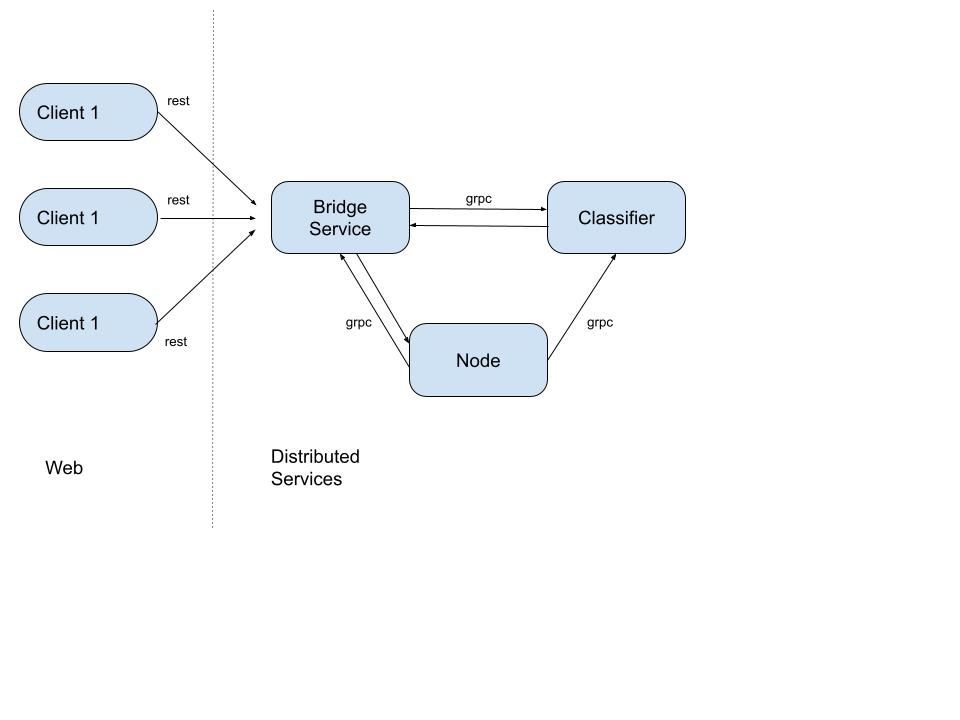
\includegraphics[width=16cm]{Esquema_puente.jpg}
		\subsection{Varias instancias no pueden compartir dependencias}
			La naturaleza que adopta la red crea una jerarquía de instancias de servicios repartidas entre los nodos de la mísma. \\
			Esto significa que, cuando una instancia (padre) solicita una instancia de otro servicio (hijo), este último
			pasará a ser dependiente del primero, adoptando el padre el derecho a decidir cuando debe de morir el hijo y la responsabilidad
			sobre su consumo de recursos (en caso en que un nodo realice un seguimiento del consumo de cada instancia, deberá tener en cuenta el de sus dependencias).
			De esta forma, si se mata al padre, el nodo donde se este ejecutando su hijo podrá matarlo. \\
			Si no fuera asi, un nodo no sabría que instancias quedan en estado 'zombie' ya que ninguno de sus clientes 
			(instancias padre) se haría responsable.

		\subsection{Comunicación nodo-servicio}
			Definir como debe comportarse un sistema requiere abordar cuales son los deberes y derechos de sus componentes. \\
			Un nodo debe de proporcionar una interfaz con la que los servicios puedan comunicarse, junto con la dirección
			a la que el servicio le realizará sus solicitudes. La forma en la que el nodo carga estos componentes en una nueva instancia
			es mediante un archivo binario en la raíz del sistema de ficheros del servicio. Esto es así ya que el servicio podría requerir de
			estos datos antes de levantar su servidor. \\
			Ante la solicitud de una nueva instancia, un nodo tiene el derecho de, o bien construir esta instancia localmente, o bien solicitarle la instancia
			a un par (otro nodo). Así mismo, el nodo tiene el deber de retornar tanto una dirección con la que comunicarse con la nueva instancia, como un token
			para realizar acciones sobre ella al solicitante.
			En caso de crear la dependencia de un servicio en un par, el nodo debe de asegurarse que el solicitante tenga acceso a la dirección que le otorga para
			comunicarse con su dependencia. \\
			Esta arquitectura permite a un servicio no preocuparse del nodo donde se ejecutará cada dependencia. Del mismo modo que los nodos no se preocuparán de
			la utilidad que puedan tener las instancias que ejecutan. \\
			Por tanto, para resumir, durante la construcción de la instancia de un servicio, el nodo añade en su raíz un binario que contiene como comunicarse con él.
			Si el servicio quiere dar uso de una dependencia, le enviará la especificación de ésta al nodo, y éste le devolverá una dirección con la que comunicarse y
			un token para poder matarla. Será el nodo el que busque donde construir esa dependencia, si localmente o en alguno de sus pares. También será el nodo el que,
			en caso de matar a la primera instancia, acabe con la segunda.

		\subsection{Serialización y topología de la especificación de un servicio}
			La especificación de un servico se serializa en un binario Protobuf. \\

			Está compuesto por los siguientes elementos:
			\begin{itemize}
				\item hash: Lista de hashes (del tipo sha256:913ref3...) sobre el binario del resto de la especificación.
				\item Syntax: Sintaxis de la especificación.
				\item Container: Especifica el contenedor donde se ejecuta el servicio, esto es:
					\begin{itemize}
						\item la arquitectura, define el hardware y el kernel donde se debe de ejecutar el servicio.
						\item el punto de entrada, define la ruta del primer ejecutable del servicio.
						\item el sistema de archivos, representado en un árbol donde las hojas son los archivos en binario.
						\item las variables de entorno, lista compuesta por llave y definición del campo de cada variable. 
					\end{itemize} 
				\item Api: Define cómo se puede interactuar con el servicio, constituida por:
					\begin{itemize}
						\item interfaz de la aplicación (mensajes, métodos y errores y respuestas de cada uno).
						\item lista de slots, cada uno compuesto por los siguentes elementos:
							\begin{itemize}
								\item puerto donde escucha.
								\item protocolo de comunicación que soporta (HTTP/2, GRPC ...).
							\end{itemize}
					\end{itemize} 
				\item Tensor: Opcional. Definie la topología del modelo que entrena el servicio. Un servicio podría solicitar al nodo que le retorne las instancias
					de aquellos servicios que tengan un tensor determinado y con ellas realizar solicitudes a servicios que ya tienen el modelo entrenado.
			\end{itemize}
		\subsection{Json vs GRPC} 
			Json se ha convertido en prácticamente un estándar a la hora de compartir información en la web, debido a que es el sistema de serialización de Javascript, y éste, a su vez,
			es el lenguaje estandarizado para ejecutarse en los navegadores web. \\

			Pero en una red de microservicios, donde los entornos de ejecución son virtualizados, Javascript pierde protagonismo y, por tanto, Json también.
			Es por esto que cabe preguntarse cual es la mejor forma de serializar las comunicaciones entre servicios. Al ser evidente que no existe un protocolo capaz de
			liderar ni en cualquier ámbito ni indefinidamente, cada Slot de un servicio definirá el protocolo soportado. \\

			Concretamente para este proyecto se dará uso de Grpc, principalmente por dos razones:
			\begin{itemize}
				\item Protobuf, su lenguaje de serialización, consigue comprimir bytes de manera muy eficiente enfocando los buffers a cada topología de mensajes.
				\item Utiliza Http/2, por lo que está preparado para realizar streaming bidireccional de manera eficiente.
			\end{itemize}
			Otros protocolos también a tener en cuenta podrían ser Flatbuffers o Capt'n proto.

	\section{Resultados y conclusiones}
	\section{Trabajo futuro}

	\bibliography{referencies}
	\bibliographystyle{plain}
	\nocite{*}
\end{document}